\chapter{Introduction}
\label{ch:intro}

The realm of nuclear security involves parallel efforts in nonproliferation
(verification of treaty compliance, monitoring for smuggling, proper storage
and transportation of nuclear materials), cyber security, minimizing stocks of
weaponizable materials, disaster response training, and nuclear forensics. All
of these efforts have been continually improving, but there was a gap regarding
the ability of the \gls{US} to coordinate and respond to a nuclear incident,
especially with the technical portion of nuclear forensics: characterization
and analysis. After all, the first textbook on the topic was published in 2005
\cite{nftext_2005}. In 2006, the \gls{US} \gls{DHS} founded the \gls{NTNFC}
within the \gls{DNDO}. The mission of the \gls{NTNFC} is to establish a robust
nuclear forensics capability to attribute radioactive materials with
demonstrable proof. In 2017, the \gls{DNDO} was absorbed into the newer
\gls{CWMD} Office.

Multiple fields contribute to a nuclear forensics capability, such as
radiochemical separations, material collection techniques, detector technology,
material library development, and identifying forensic signatures. These needs
vary based on whether the material being collected is post-detonation (e.g.,
bomb debris) or pre-detonation (e.g., \glsreset{SNF}).  In the pre-detonation
realm, this project focuses on statistical methods to to model \gls{SNF}
production history using nondestructive detector measurements. 

\section{Motivation}
\label{sec:motivation}

Nuclear forensics is an important aspect of deterring nuclear terrorism even
though it is not, at first glance, obvious preventative nuclear security.  The
most common defense of the field is that nuclear forensics deters state actors,
not terrorist organizations. While it is true that a strong capability
encourages governments to be more active in prevention of nuclear terrorism, it
can also deter the terrorist organizations as well by increasing their chances
of failure. Small destructive successes tend to be more valued than high-risk
mass destruction. Nuclear forensics can also assist in cutting off certain
suppliers of nuclear materials or technologies (e.g., nuclear specialists that
are only involved for financial reasons, access to state suppliers), building a
concrete barrier to nuclear terrorism.  Therefore, nuclear forensics is
considered to impede nuclear terrorism in both tangible and abstract ways
\cite{aps_aaas_forensics}.

Following the prevention value of nuclear forensics, it is important to
understand the process of the technical portion of the investigation and how
that can be improved.  In the event of a nuclear incident, such as the
retrieval of stolen \gls{SNM} or the detonation of a dirty bomb, it is
necessary to learn as much as possible about the source of the materials in a
timely manner. In the case of non-detonated \gls{SNM}, knowing the processes
that produced it is crucial to determine the chain of custody of the
interdicted material.  Section \ref{sec:nfneeds} covers the specific needs of
the nuclear forensics community for \gls{SNF} provenance, and Section
\ref{sec:statscontrib} discusses how computational approaches are useful, with
a focus on why statistical methods in particular are being pursued. 

\subsection{Needs in Nuclear Forensics}

\begin{frame}
  \frametitle{Nuclear Forensics Investigations}
  \begin{minipage}[t]{0.5\textwidth}
    \textbf{Post-detonation}
    \begin{itemize}
      \item Collection: debris, swipe samples
      \item Characterization: rapid analysis of isotope ratios
      \item Goals
      \begin{itemize}
        \item Inverse problem: reconstruct weapon design/yield
        \item Safety: informing disaster response
      \end{itemize}
      \item Data evaluation
    \end{itemize}
  \end{minipage}%
  \pause
  \begin{minipage}[t]{0.5\textwidth}
    \textbf{Pre-detonation}
    \begin{itemize}
      \item Collection: depends on intercepted material
      \item \boxalert{Characterization:} non-destructive and destructive
      \item Goals:
      \begin{itemize}
        \item \boxalert{Inverse problem:} material chain of custody
        \item Safety: material handling and security
      \end{itemize}
      \item \boxalert{Data evaluation}
    \end{itemize}
  \end{minipage}
\end{frame}


\begin{frame}
  \frametitle{Nuclear Forensics as an Inverse Problem}
  Necessary to determine the quality of prediction

  Use Bayes' Framework:
  $$ P(A|B) = \frac{P(B|A)P(A)}{P(B)} $$
  $$ P(M|D) = \frac{P(D|M)P(M)}{P(D)} $$
\end{frame}


\label{sec:nfneeds}

\subsection{Contribution of Statistical Methods}
As previously mentioned, there are two main issues that are being addressed for
forensics of \gls{SNF}: database issues and speed of characterization. Many
have begun considering computational approaches to nuclear forensics problems,
such as the INDEPTH tool for inverse depletion and decay analysis
\cite{weber_2006, weber_2010, weber_2011}. This tool uses an iterative
optimization method involving many forward simulations to obtain reactor
parameters of interest given some initial values. 

Another approach utilizes artificial intelligence to solve nuclear forensics
problems, such as implementing searching algorithms for the database comparison
step \cite{gey_search} and machine learning for determining reactor parameters
from \gls{SNF} characteristics \cite{dayman_feasibility_2013, nicolaou_2006,
nicolaou_2009, nicolaou_2014, robel_2009, jones_viz_2014, jones_snf_2014}.  A
variety of statistical and machine learning tools have been used to
characterize spent fuel by predicting categories or labels (reactor type, fuel
type) as well as predicting values (burnup, initial enrichment, or cooling
time) The former uses classification algorithms and the latter uses regression
algorithms. Many algorithms can be applied to both cases.

A typical (supervised) machine learning workflow would take a set of training
data with labels or values inserted into some statistical learner, calculate
some objective, minimize or maximize that objective, and provide some model
based on that output. Then a test set (with known values) is provided to the
model so that its performance can be evaluated and finalized. After model
finalization, a user can provide a single instance and a value can be predicted
from that. \todo{insert ML schematic}

To obtain reliable models, one must 1. choose/create a training set carefully
and 2. study the impact of various algorithm parameters on the error. Many
algorithms are developed on an assumption that the training set will be
independent and identially distributed (i.i.d.). [Aside: there are ways to
handle skewed data sets] This is important so that the model does not overvalue
or overfit a certain area in the training space. Additionally, algorithm
performance (or error) can be optimized with respect to training set size,
number of features, or algorithm parameters (regularization terms, etc).  These
are known as diagnostic plots. When plotting the training and testing error
with respect to the number of instances, this is known as a learning curve.
When plotting these errors with respect to the number or features or algorithm
parameters, this is known as a validation curve. \todo{insert example
diagnostic plot?}

Algorithm choice is usually based on what is being predicted and intuition
regarding strengths and weaknesses.  For the sake of comparison (i.e. weak
validation), some machine learning approaches here are based on previous work
\cite{dayman_feasibility_2013} while also extending to a more complex model
via an algorithm that is known to handle highly dimensional data sets well.
Thus, this paper investigates three regression algorithms: nearest neighbor,
ridge, and support vectors.


It is first important to determine if statistical methods can
overcome the inherent database deficiencies. Next, the statistical methods must
be considered in such a way as to represent a real-world scenario. Although
mass spectrometry techniques provide extremely accurate isotopic information
for analytical methods, they are time-consuming and more expensive. And
although gamma spectroscopy can give extremely fast results cheaply, it only
measures certain radiological signals and is influenced by many environmental
factors, storage, and self-attenuation. As different machine learning
algorithms and parameters are investigated, this work focuses on probing the
amount of information required to obtain realistic results.

Because creating databases from real measurements to represent reactor
technologies from around the world is impossible, the database in this study
will be created from high-fidelity simulations via ORIGEN irradiation and
depletion \todo{check actual name of code part used}. In the simulation and
statistical learning paradigm, we need to determine how much information to
what quality is needed to train a machine-learned model; the model must give
appropriate predictions of reactor parameters given a set of measurements from
a test sample of interdicted \gls{SNF}. Of interest to an entity trying to
create a weapon is partially irradiated fuel if they have plutonium separations
capabilities or any radioactive substance in the case of a dirty bomb.
Addressing the former, a set of simulations of \gls{SNF} at different burnups
and cooling times will comprise the database.\todo{rewrite to be clearer}

Can the algorithm overcome the deficiencies of gamma detection and still
provide useful results? Or does it need more information, e.g., exact
isotopics? First, we must establish some baseline expectations of reactor
parameter prediction and how different algorithms perform. This work is based
off previous work on the subject \cite{dayman_feasibility_2013} regarding
machine learning performace with respect to information reduction, and expands
upon it by also evaluating a more advanced machine learning algorithm: support
vector regression. 



Below is a more in depth discussion of nuclear forensics and
how machine learning can contribute to this research area. After that, an
experimental design is outlined. Lastly, the results are presented and
discussed. 

Thus, ultimately, the goal is to answer the question \textit{How
does the ability to determine forensic-relevant spent nuclear fuel attributes
degrade as less information is available?}. 

%%%%%



\label{sec:statscontrib}

\section{Methodology}
\label{sec:methodology}

As previously mentioned, the typical workflow of the technical portion of a
forensics investigation is to analyze measurements of an unknown material. The
measurements are compared to databases filled with previously measured standard
materials with known reactor parameters, and/or the reactor parameters are
calculated from empirical relationships.  As this work focuses on \gls{SNF},
these measurements are elemental, chemical, and radiological in nature.
Because creating databases from real measurements to represent \gls{SNF} from
reactor technologies from around the world is not within the scope of this
project, the database in this study will be created from high-fidelity
simulations via the \gls{SCALE} \cite{scale} system using \gls{ORIGEN}
\cite{origen}. 


To understand how a physics-free model can predict nuclear reactor parameters,
Figure \ref{fig:compworkflow} introduces two computational workflows. Both the
\gls{INDEPTH} and statistical methodologies begin with simulated \gls{SNF}.
While not all steps are required to be equivalent, the only difference here is
the method one chooses to obtain reactor parameters. Both workflows address
speed of characterization, as it is intended to have gamma spectra as the
inputs.  Because \gls{INDEPTH} is better studied and validated than statistical
methods \cite{weber_2006, weber_2011, weber_2010}, this work focuses on a
statistical approach but with the intention to compare methodologies.  Both
workflows also address many of the database issues, described above. The
statistical methodology using \gls{ML} is described below.
\\
\begin{figure}[!tbh]
  \makebox[\textwidth][c]{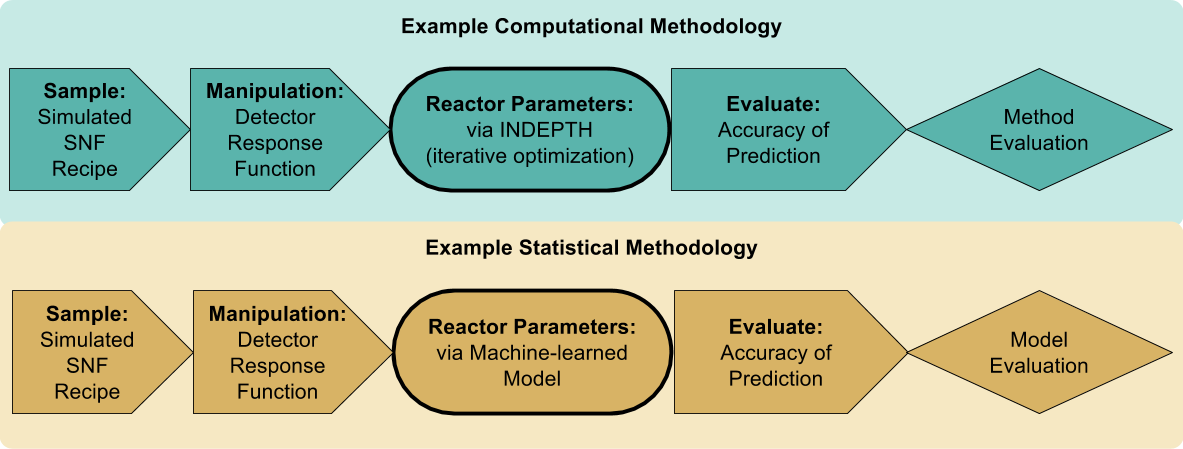
\includegraphics[width=\linewidth]{./chapters/intro/CompStatForensicsWorkflow.png}}
  \caption{Computational Forensics Research Workflows}
  \label{fig:compworkflow}
\end{figure}

In the simulation and statistical learning paradigm, we need to determine how
much information to what quality is needed to train an \gls{ML} model;
the model must give appropriate predictions of reactor parameters given a set
of measurements from a \textit{test} sample. 
\todo[inline]{a bit out of place; maybe delete} 

After creating a set of gamma spectra corresponding to simulations of \gls{SNF}
resulting from chosen reactor operation conditions, the next step is to choose
an algorithm that performs model creation via statistical learning.
Statistical learners have varied strengths and weaknesses based on what is
being predicted and how they implement optimization.  Chosen for this study are
simple regression algorithms for burnup prediction: nearest neighbor and
decision trees.  For comparison, \acrfull{SVR} is used because it is known to
handle highly dimensional data sets well.  These algorithms are introduced in
Section \ref{sec:algs}.

After the training is complete, the results of each models' predictions must be
evaluated according to \gls{ML} best practices.  The machine-learned
model predicts the parameters of a previously unseen test set.  The difference
between the model predictions and the actual simulated parameters is known as
the testing error.  The testing error with respect to various specifications
such as the training set size, number of features, or algorithm parameters
provides insight into the model performance. These results are broadly known as
diagnostic plots and show if the predictions are due to good performance or bad
fitting. 

After the models are evaluated, it will be important to compare them both
against each other and against other computational forensics methods. Thus, a
Bayesian approach from the field of inverse problem theory will be used to give
the probability distribution of the predictions so that the statistically
generated predictions can be evaluated directly against other solutions, such
as the optimization-based method, \gls{INDEPTH}. 
\todo[inline]{This might not be possible, or robustly possible}

Next, information reduction (within the training and testing data sets) must be
used to investigate the extension of this workflow to the real world. The
primary example here is the reduction of information quality via gamma ray
detectors.  If an algorithm could overcome the limitations of gamma detection
and still provide useful results, this would warrant further studies and
perhaps be field-applicable.

Thus, ultimately, the goal is to answer the question \textit{How does the
ability to determine forensic-relevant spent nuclear fuel attributes using
statistical techniques degrade as less information is available?}. 

\section{Goals}

The main purpose of this work is to evaluate the utility of statistical methods
as an approach to determine nuclear forensics-relevant quantities as less
information is available. \Gls{ML} algorithms are used to train models to
provide these values (e.g., reactor type, time since irradiation, burnup) from
the available information, or statistical methods are used for probabilistic
matching.  The training data is simulated using \gls{ORIGEN}, which provides an
array of nuclide concentrations as the features ($X$) and the parameters of
interest ($y$) are provided from the simulation inputs.  Information reduction
is carried out using computationally generated gamma spectra; the radionuclide
concentrations from the simulations can be converted into gamma energies, which
then undergo a detector response calculation to represent real as-measured
gamma spectra as closely as possible.  \Gls{ML} best practices are used to
evaluate the performance of the chosen algorithms, and inverse problem theory
is used to provide an interval of confidence in the model predictions.
\todo[inline]{update me if necessary}

The necessary background is covered in Chapter \ref{ch:litrev}.  First, an
introduction to the broader field of nuclear forensics is in Section
\ref{sec:nfoverview} to place this work in the context of the technical mission
areas. After that, a short discussion of the field of \gls{ML}, the algorithms
used, and validation methods are in Section \ref{sec:mlback}.
\todo[inline]{this will have to be reworded after the lit review is updated}
Section \ref{sec:fcsim} includes information about the software used to
generate the training data and perform the predictions. Lastly, a review of
statistical methods being used in studies of forensics analysis is covered in
Section \ref{sec:stats4nf}. 

...........................................................................
\todo[inline]{Update after research chapters are flushed out}

After the existing work is discussed, the methodology and a demonstration of
the experimental components is introduced next in Chapter \ref{ch:demo_method}.
This will cover the simulated training data in Section \ref{sec:training}, the
the details for training models in Section \ref{sec:statmodel}, and the
process of model evaluation in Section \ref{sec:valid}.  

Finally, Chapter \ref{ch:proposal} summarizes the official thesis research
proposal. After the preparatory tasks are covered in Section \ref{sec:prep},
there are three experiments outlined in Sections \ref{sec:exp1},
\ref{sec:exp2}, and \ref{sec:exp3}. Qualitiative hypotheses as well as
alternative directions for risk mitgation are discussed throughout these
sections.  A detailed explanation of the method comparison step is covered next
in Section \ref{sec:modelcompare}.  Lastly, a projected timeline for the
completion of this project is in Section \ref{sec:timeline}.
